\section{Anisotropy Invariant Analysis}
\label{ch:anisotropy}

Open from `3.\ Analysis $\to$ Anisotropy Invariants`.

\begin{quote}
\textbf{Note}
This module requires \textbf{stereo PIV (2D3C)} data. It is not available for 2D2C datasets.
\end{quote}

The Reynolds stress tensor $b_{ij} = \langle u'_i u'_j \rangle / (2k) - \delta_{ij}/3$ is a symmetric, traceless tensor that describes the anisotropy of the turbulence. Its eigenvalues $\lambda_1 \geq \lambda_2 \geq \lambda_3$ satisfy $\lambda_1 + \lambda_2 + \lambda_3 = 0$. The invariants of $b_{ij}$,
\[
\eta^2 = \frac{1}{6} b_{ij} b_{ji}, \qquad \xi^3 = \frac{1}{6} b_{ij} b_{jk} b_{ki},
\]
define a two-dimensional state space. All physically realizable turbulence states lie within the Lumley triangle, bounded by the one-component ($\lambda_1 = 2/3$), two-component ($\lambda_3 = -1/3$), and isotropic ($\lambda_i = 0$) limits (Lumley, 1978). The barycentric map is an alternative linear representation of the same anisotropy state space introduced by Banerjee et al.\ (2007), which maps the three limiting states to the vertices of an equilateral triangle with coordinates that vary linearly between limits.

\noindent\textbf{References:} Lumley, J.L. (1978). Computational modeling of turbulent flows. \textit{Advances in Applied Mechanics}, 18, 123--176. Banerjee, S., Krahl, R., Durst, F. \& Zenger, Ch. (2007). Presentation of anisotropy properties of turbulence. \textit{International Journal of Heat and Fluid Flow}, 28(3), 939--946.

\subsection{Lumley triangle mode}

\begin{quote}
\textbf{Important}
\begin{enumerate}[leftmargin=1.5em, topsep=2pt]
  \item Ensure `Line (Lumley triangle)` is selected.
  \item Choose `Free`, `Horizontal`, or `Vertical` line orientation.
  \item Left-click and drag on the mean field to draw the sampling line.
  \item Click `Compute`.
\end{enumerate}
\end{quote}

Reading the triangle: the top vertex represents one-component turbulence; the bottom-left vertex represents two-component axisymmetric (disk-like) turbulence; the bottom-right vertex represents two-component axisymmetric (rod-like) turbulence; the origin represents isotropic turbulence. Points outside the boundary indicate numerical issues (insufficient snapshots or masked regions).

\begin{figure}[htbp]
  \centering
  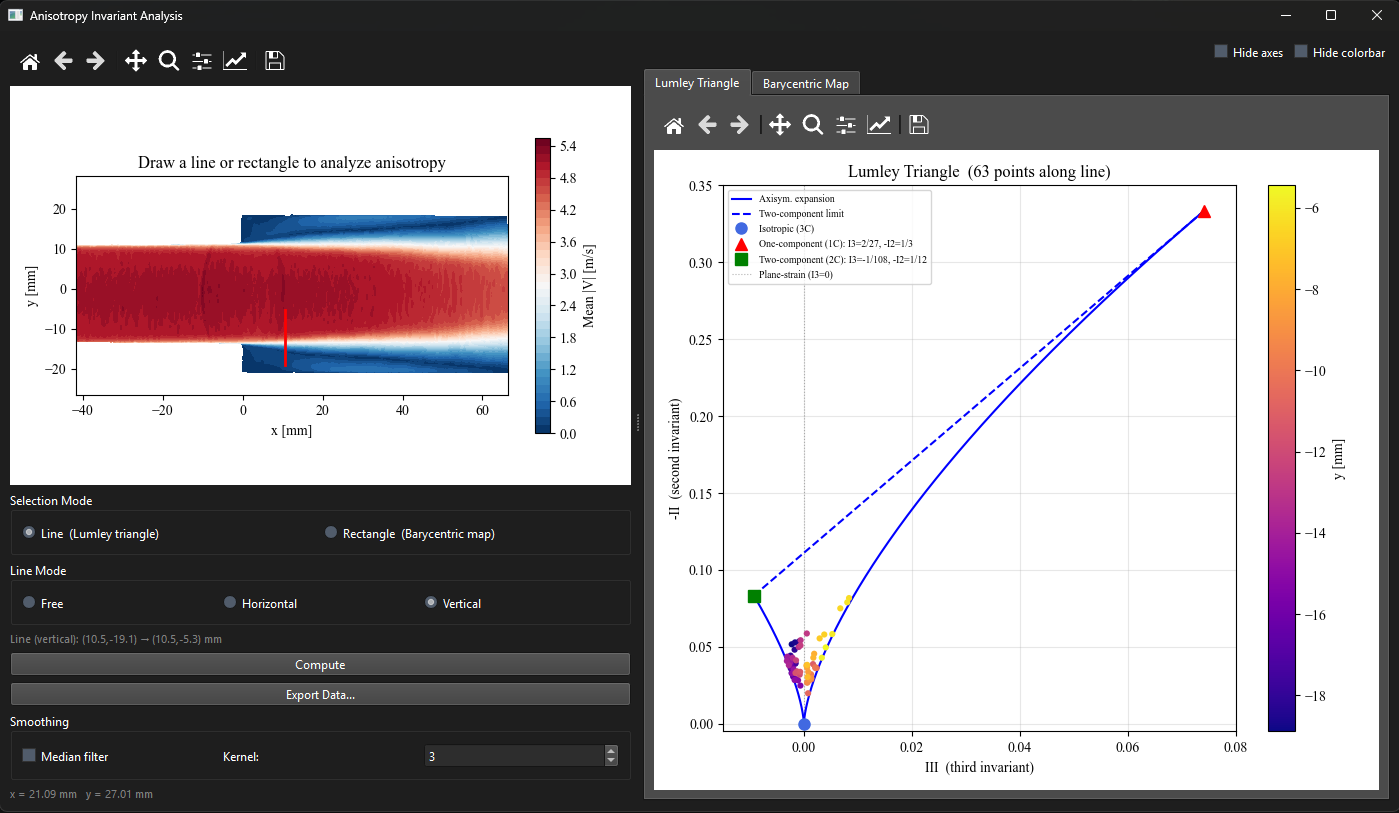
\includegraphics[width=0.92\linewidth]{fig7}
  \caption{Anisotropy window in Lumley triangle mode. Left: the vertical sampling line crosses the shear layer on the mean field. Right: each sampled point appears in the triangle, colored by its distance along the line. Points migrate from near-isotropic (center) toward the one-component vertex (top) inside the high-turbulence shear layer.}
  \label{fig:anisotropy}
\end{figure}

\subsection{Barycentric map mode}

\begin{quote}
\textbf{Important}
\begin{enumerate}[leftmargin=1.5em, topsep=2pt]
  \item Select `Rectangle (Barycentric map)`.
  \item Left-click and drag to draw a rectangular region on the field.
  \item Click `Compute`.
\end{enumerate}
\end{quote}

The map colors each grid point by its anisotropy state: red = one-component, blue = two-component axisymmetric, green = three-component (near isotropic). Check `Median filter` to apply a $3\times3$ spatial smoothing to reduce noise.

\subsection{Multi-case comparison}

Lumley-triangle line profiles support CSV import and overlay (Chapter~\ref{ch:multicase}).

% ============================= CHAPTER 9 ==============================
